\chapter{Conventions And Notations}
\section{Notations}
Let us introduce notations that will be kept all along the report:
\begin{itemize}
  \item $M$ refers to a bit string of arbitrary length, i.e. $M \in {\{0,1\}}^*$.
  \item $\vert M\vert$ denotes the bit-length of M.
  \item $A\vert \vert B$ denotes the concatenation of $A$ and $B$, where $A, B \in {\{0,1\}}^*$.
  \item $ M\vert \vert pad\lbrack r\rbrack (\vert M\vert )$ denotes the padding of a message M that is to be split into blocs of $r$ bits.
  \item $\vert M\vert_r$ denotes the number of blocs  of $r$ bits that M splits into once padded.
  \item $\lfloor M\rfloor_r$ denotes the truncation of a bitstring M to its first $r$ bits, $r\in \mathbb{N}$.
  \item For $a, b \in \mathbb{N}$, the notation  $\llbracket a,b \rrbracket$ is used to indicate the interval of all integers between a and b, including both. To indicate that one of the endpoints is to be excluded from the set, the corresponding square bracket is reversed.
  \item For a given set $\mathcal{E}$, $\# \mathcal{E}$ is the cardinal of $\mathcal{E}$.
\end{itemize}

\section{Padding Rules}\label{section:padding}

As we will see later on, in Section~\ref{sec:MerkleDamg}, hashing functions are iterated compression functions, which are applied to fixed length bit strings.
Seeing as the input of a hash function can be a message of any length,
it needs to be split into a number of sub-messages, called blocks, of a given length, so that the compression function can be applied to each block.

Of course the length of the message is not always an exact multiple of the required block length. 
In order to deal with this length problem, the input message is padded, so as to obtain the required length.
Note that the choice of the padding rule is extremely important as a poor choice may render the hashing algorithm cryptographically insecure.

\begin{defn} \emph{Simple padding}, denoted by pad10∗, appends a single bit 1 followed by the minimum number of bits 0 such that the length of the result is a multiple of the block length.
Simple padding appends at least 1 bit and at most the number of bits in a block. 
\end{defn}

\begin{figure}[H]
  \centering
  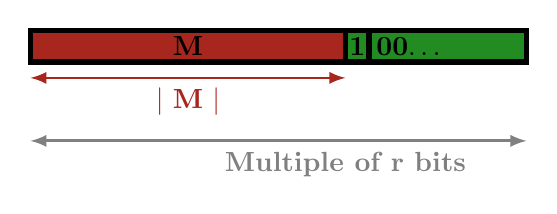
\begin{tikzpicture}[scale=1]
    
    \draw [name=green, fill=Mahogany, line width=2pt] (0,0) rectangle (4,0.4);
    \draw [fill=ForestGreen, line width=2pt] (4,0) rectangle (4.3,0.4);
    \draw [fill=ForestGreen, line width=2pt] (4.3,0) rectangle (6.3,0.4);

    \node [align=center] at (2,0.2){\textbf{M}};
    \node [align=center] at (4.15,0.2){\textbf{1}};
    \node [align=left]   at (4.8,0.2){\textbf{00}$\ldots$};
    
    \draw [<->, >=latex, line width=1pt, color=Mahogany] (0,-0.2) -- (4,-0.2);
    \draw [<->, >=latex, line width=1pt, color=Gray] (0,-1) -- (6.3,-1);

    \node [align=center, color=Mahogany] at (2,-0.5){$\vert$ \textbf{M} $\vert$};
    \node [align=center, color=Gray] at (4,-1.3){\textbf{Multiple of r\ bits}};
    
  \end{tikzpicture}
  \caption{\label{fig:SimplePadding}Simple padding.}
\end{figure}

Hashing functions based on the Merkle-Damg\r{a}rd construction, as defined in Section~\ref{sec:MerkleDamg}, use a similar padding rule to \emph{simple padding}. Simple padding is applied to obtain a message length of $r-64$ bits, after which the binary length of the original message, encoded as a 64-bit long integer, is appended to the padded message. The resulting length of the padded message $ M\vert \vert pad\lbrack r\rbrack (\vert M\vert )$ is $r\cdot \vert M\vert_{r}$ where $\vert M\vert_{r}$ is a positive integer (cf Figure~\ref{fig:MDPadding}).
\begin{figure}[H]
  \centering
  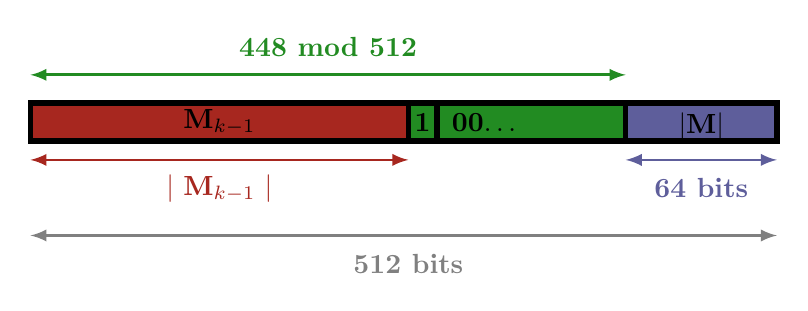
\begin{tikzpicture}[scale=1.2]
    
    \draw [name=green, fill=Mahogany, line width=2pt] (0,0) rectangle (4,0.4);
    \draw [fill=ForestGreen, line width=2pt] (4,0) rectangle (4.3,0.4);
    \draw [fill=ForestGreen, line width=2pt] (4.3,0) rectangle (6.3,0.4);
    \draw [fill=MidnightBlue!70, line width=2pt] (6.3,0) rectangle (7.9,0.4);

    \node [align=center] at (2,0.2){\textbf{M$_{k-1}$}};
    \node [align=center] at (4.15,0.2){\textbf{1}};
    \node [align=left]   at (4.8,0.2){\textbf{00}$\ldots$};
    \node [align=center] at (7.1,0.15){$\vert \textbf{M}\vert $};
    
    \draw [<->, >=latex, line width=1pt, color=Mahogany] (0,-0.2) -- (4,-0.2);
    \draw [<->, >=latex, line width=1pt, color=ForestGreen] (0,0.7) -- (6.3,0.7);
    \draw [<->, >=latex, line width=1pt, color=Gray] (0,-1) -- (7.9,-1);
    \draw [<->, >=latex, line width=1pt, color=MidnightBlue!70] (6.3,-0.2) -- (7.9,-0.2);

    \node [align=center, color=Mahogany] at (2,-0.5){$\vert$ \textbf{M$_{k-1}$} $\vert$};
    \node [align=center, color=ForestGreen] at (3.15,1){\textbf{448\ mod\ 512}};
    \node [align=center, color=Gray] at (4,-1.3){\textbf{512\ bits}};
    \node [align=center, color=MidnightBlue!70] at (7.1,-0.5){\textbf{64\ bits}};
    
  \end{tikzpicture}
  \caption{\label{fig:MDPadding}Merkle-Damg\r{a}rd padding.}
\end{figure}

For alternative hashing functions based on the sponge construction, as defined in Section~\ref{sec:Sponge}, we introduce an additional security constraint:
\begin{defn}A padding rule is \emph{sponge-compliant} if it never results in the empty string and if it satisfies following criterion:
$$\forall n \ge 0\mbox{, } \forall M, M' ∈ \mathbb Z_2^* \mbox{: } M \ne M′ \Rightarrow \mbox{ }M\vert \vert pad \lbrack r\rbrack(\vert M\vert ) \ne M'\vert \vert pad\lbrack r \rbrack (\vert M'\vert )\vert \vert 0^{nr}$$
\end{defn}

\emph{Simple padding} is the simplest padding rule that is sponge-compliant. The simplest padding rule that allows securely using the same f with different rates is the following:
\begin{defn} \emph{Multi-rate} padding, denoted by pad10∗1, appends a single bit 1 followed by the minimum number of bits 0 followed by a single bit 1 such that the length of the result is a multiple of the block length.
Clearly, this padding rule is sponge-compliant as well as it is injective and cannot result in an empty string or a string with all-zero last block. Multi-rate padding appends at least 2 bits and at most the number of bits in a block plus one.
\end{defn}


\begin{figure}[H]
  \centering
  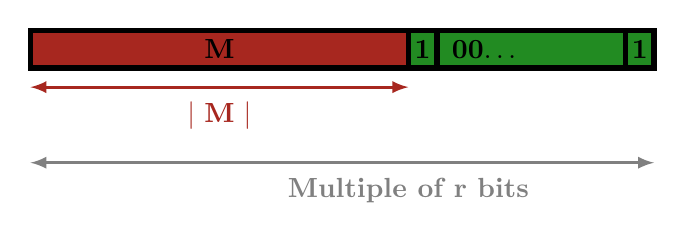
\begin{tikzpicture}[scale=1.2]
    
    \draw [name=green, fill=Mahogany, line width=2pt] (0,0) rectangle (4,0.4);
    \draw [fill=ForestGreen, line width=2pt] (4,0) rectangle (4.3,0.4);
    \draw [fill=ForestGreen, line width=2pt] (4.3,0) rectangle (6.3,0.4);
    \draw [fill=ForestGreen, line width=2pt] (6.3,0) rectangle (6.6,0.4);

    \node [align=center] at (2,0.2){\textbf{M}};
    \node [align=center] at (4.15,0.2){\textbf{1}};
    \node [align=left]   at (4.8,0.2){\textbf{00}$\ldots$};
    \node [align=center] at (6.45,0.2){\textbf{1}};
    
    \draw [<->, >=latex, line width=1pt, color=Mahogany] (0,-0.2) -- (4,-0.2);
    \draw [<->, >=latex, line width=1pt, color=Gray] (0,-1) -- (6.6,-1);

    \node [align=center, color=Mahogany] at (2,-0.5){$\vert$ \textbf{M} $\vert$};
    \node [align=center, color=Gray] at (4,-1.3){\textbf{Multiple of r\ bits}};
    
  \end{tikzpicture}
  \caption{\label{fig:MultiPadding}Multi-rate padding.}
\end{figure}

